% =====================================================================================
%  Restoring fault distance three in magic state cultivation under the hardware
%  constraints of a superconducting processor
%
%  Draft v0.1 (Nov 9, 2026). Compile with pdfLaTeX + BibTeX (Overleaf: default settings).
%  Every number in this draft is taken from the result files listed in README.md.
%  Lines marked  % TODO  need the authors' input.
% =====================================================================================
\documentclass[aps,pra,reprint,superscriptaddress,longbibliography]{revtex4-2}

\usepackage[utf8]{inputenc}
\usepackage[T1]{fontenc}
\usepackage{amsmath,amssymb,amsfonts}
\usepackage{graphicx}
\usepackage{booktabs}
\usepackage{xcolor}
\usepackage[colorlinks=true,linkcolor=blue!60!black,citecolor=blue!60!black,urlcolor=blue!60!black]{hyperref}

\newcommand{\ket}[1]{\left|#1\right\rangle}
\newcommand{\HXY}{H_{XY}}
\newcommand{\df}{d_{\mathrm{f}}}
\newcommand{\csz}{\textsf{cs02}}
\newcommand{\Gfour}{\textsf{G4}}
\newcommand{\Gsix}{\textsf{G4-G6}}
\newcommand{\todo}[1]{\textcolor{red}{[TODO: #1]}}

\begin{document}

\title{Restoring fault distance three in magic state cultivation\\under the hardware constraints of a superconducting processor}

% The affiliation text (with the e-mail line) is defined once and used for every author with this
% affiliation, so it is printed once, under the author list and above the abstract.
\newcommand{\affPKNU}{\todo{Department}, Pukyong National University, Busan, Republic of Korea\\
Corresponding author: \href{mailto:sokpheng001@pukyong.ac.kr}{\texttt{sokpheng001@pukyong.ac.kr}}}

\author{Kim Chansokpheng}
\affiliation{\affPKNU}

\author{\todo{Co-author / advisor}}
\affiliation{\affPKNU}

\date{\today}

\begin{abstract}
Magic state cultivation prepares high-fidelity $T$ states at a cost comparable to a logical CNOT and has recently been demonstrated on Google's Willow processor.
Its central gadget, the double check of the logical operator $\HXY$ on the distance-3 colour code, is designed for fault distance three, but with physical $T$ gates hook errors become Clifford errors and the fault distance of one double check drops to two, including for the circuit run on hardware.
Flag qubits that restore the fault distance exist, but they need next-nearest-neighbour couplings and do not fit a square-lattice device.
We formulate the design of the double check as a constrained search under the constraints of Willow: nearest-neighbour couplings only, at most four coupling partners per qubit, and a readout-line rule under which no measured qubit may share a readout line with a data qubit that must survive into the next stage.
The search returns \csz, a 12-qubit double check with 24 two-qubit gates, two flags and fault distance three with real $T$ gates, verified by exhaustive fault enumeration and by fault injection in Google's quantum virtual machine.
Against Google's own double check, run in the way it must run when the cultivated state continues, \csz\ lowers the error per kept $T$ state from 1 in 20,832 to 1 in 121,322 (5.8 times, 95\,\% interval 4.2--8.1) at nearly the same acceptance (75.2\,\% against 76.7\,\%), in Google's simulator of Willow.
The gain is 3.0--5.7 times across four further noise models, grows as $1/p$ as the physical error rate $p$ falls (13.7 times at $p=0.05\,\%$), and is 2.3 times in the median over all valid chip placements.
We check our simulation chain against Google's released hardware data: our analysis reproduces the paper's figures from the raw shots, the baseline is gate for gate the circuit that was run, and the simulator agrees with the hardware retention to within 6\,\%.
The same method gives distance-5 double checks with fault distance four that fit the device and lower the error 3.0--5.4 times relative to the published distance-5 design.
\end{abstract}

\maketitle

% =====================================================================================
\section{Introduction}
% =====================================================================================

Fault-tolerant quantum computers implement Clifford operations cheaply in codes such as the surface and colour codes, but no code with a transversal universal gate set exists~\cite{EastinKnill2009}.
The standard way to complete the gate set is to consume magic states such as $\ket{T}=T\ket{+}$~\cite{BravyiKitaev2005}.
Magic state distillation has long dominated the cost of fault-tolerant algorithms~\cite{Litinski2019}.
Magic state cultivation~\cite{Gidney2024cultivation} replaces distillation by a sequence of checks on a small colour code: a noisy $T$ state is injected into the distance-3 colour code, the logical operator $\HXY$, whose $+1$ eigenstate is $\ket{T}$, is measured twice (the \emph{double check}), the code may be grown and checked again, and the state finally escapes into a large surface code.
Any detection event discards the attempt.
Its expected cost is comparable to that of a logical CNOT~\cite{Gidney2024cultivation}.

Cultivation has recently been demonstrated on Google's Willow processor~\cite{Rosenfeld2025}: a $T$ state was injected and cultivated in a distance-3 colour code on a square lattice of superconducting qubits, reducing the logical error by about 40 times at a retention of 8\,\%, and the cultivated state was grafted into a distance-5 surface code.

Two recent analyses with physical (real) $T$ gates instead of the Clifford $S$-gate proxy used in sampling show that the double check does not reach its design fault distance~\cite{Chan2026diagnosing,WanZapirain2026}.
An $X$-type hook error that spreads through the CNOT fold becomes, after the physical $T$ gates, a multi-qubit Clifford error that the check does not detect.
The distance-3 (5) double check therefore has fault distance 2 (3), and the same holds for the double check that was run on hardware~\cite{Chan2026diagnosing}.
Chan \emph{et al.}\ restore the fault distance with $Z$ flags, but their flags make some interactions next-nearest-neighbour; the authors treat them as a proof of concept and list a nearest-neighbour layout, designed systematically, as an open problem~\cite{Chan2026diagnosing}.

This paper solves that problem for Willow.
Our contributions are:
\begin{enumerate}
\item A formulation of the double-check design problem under the constraints of a square-lattice device: nearest-neighbour two-qubit gates, at most four partners per qubit, and a readout-line rule that also holds when the data qubits continue into the next stage (Sec.~\ref{sec:model}).
\item \csz, a 12-qubit distance-3 double check with two nearest-neighbour flags and fault distance three with real $T$ gates, the same qubit count and two-qubit gate count as Google's circuit (Sec.~\ref{sec:cs02}).
\item A comparison with Google's hardware circuit in Google's own simulator of Willow and under four further noise models, a noise-strength sweep that confirms the fault distance, and a study over all valid chip placements (Sec.~\ref{sec:results}).
\item A validation of the simulation chain against Google's released hardware data (Sec.~\ref{sec:validation}).
\item An extension to distance 5 (Sec.~\ref{sec:d5}).
\end{enumerate}
Throughout, we compare only circuits that can run on the device; circuits that need non-neighbour couplings are discussed as motivation but not used as baselines.

% =====================================================================================
\section{Background}
\label{sec:background}
% =====================================================================================

\subsection{The double check}

The distance-3 colour code is the Steane code~\cite{Steane1996}: seven data qubits on a triangle of three plaquettes, each plaquette carrying an $X$ and a $Z$ stabiliser.
Its transversal gates include the logical $H$ and $S$, and a layer of physical $T$ and $T^\dagger$ gates on the two sublattices implements the logical $T$ up to a Clifford correction~\cite{BombinMartinDelgado2006,Gidney2024cultivation}.
The logical operator
\begin{equation}
\HXY = \frac{X+Y}{\sqrt{2}} = T\,X\,T^\dagger
\end{equation}
has $\ket{T}$ as its $+1$ eigenstate, so measuring $(\HXY)_L$ and keeping only the outcome $+1$ projects a noisy encoded state onto $\ket{T_L}$.
The measurement is built as $T_L^\dagger$, then a CNOT \emph{fold} that collects the logical $X_L$ onto a single parity (root) qubit, a single-qubit $X$ measurement of the root, the mirror-image \emph{unfold}, and $T_L$~\cite{Gidney2024cultivation}.
The double check measures the root twice, in the middle and at the end, and the helper qubits of the fold act as additional detectors after the unfold~\cite{Rosenfeld2025}.
The state is kept only if every detector is silent.

\subsection{Fault distance with real $T$ gates}

Let a fault be an error event at one circuit location.
The fault distance of the check is
\begin{equation}
\df = \min_{F\in\mathcal{F}_{\mathrm{bad}}} |F|,
\label{eq:df}
\end{equation}
where $\mathcal{F}_{\mathrm{bad}}$ is the set of fault sets that the check does not detect and that leave a wrong $T$ state; $\df$ is the size of the smallest such set.
Writing $N_k$ for the number of such malignant configurations of $k$ faults and $A(p)$ for the acceptance, the error per kept $T$ state at physical error rate $p$ is
\begin{align}
\varepsilon(p) &= \frac{\Pr[\text{kept, wrong}]}{\Pr[\text{kept}]}
  \approx \frac{1}{A(p)} \sum_{k\ge \df} N_k\,p^k \nonumber\\
&\approx N_{\df}\,p^{\df} \qquad (p\to 0).
\label{eq:eps}
\end{align}
A Pauli fault $P$ that reaches a physical $T$ gate becomes $T P T^\dagger$; for $P=Z$ this is again $Z$, but for $P=X$ it is $(X+Y)/\sqrt2$, a Clifford, non-Pauli error.
The $S$ proxy used for Clifford sampling hides this effect, which is why the proxy predicts $\df=3$ while the real circuit has $\df=2$~\cite{Chan2026diagnosing,WanZapirain2026}.
Flag qubits~\cite{ChaoReichardt2018,ChamberlandBeverland2018} that read the parity of the hook can detect the malignant pairs.

\subsection{Willow's constraints}
\label{sec:constraints}

Willow is a square lattice of transmons with tunable couplers: a qubit at row $r$ and column $c$ can perform a CZ only with its four neighbours $(r\pm1,c)$ and $(r,c\pm1)$~\cite{GoogleBelowThreshold2025}.
Qubits are read out through shared readout lines, and the layout of Google's experiment was itself chosen ``to satisfy readout line constraints''~\cite{Rosenfeld2025}.
We model the lines as the diagonals $\ell(r,c)=r+c$ and assume that measuring a qubit dephases the other live qubits on its line.
This assumption is the strict readout rule used throughout; it is consistent with the published layout but is a model, not a device specification (Sec.~\ref{sec:limitations}).

When the cultivated state is used, the seven data qubits are not measured at the end of the double check but continue into escape or grafting.
The \emph{continuing-data rule} then requires that no qubit measured during or after the check share a readout line with a data qubit.
Google's Fig.~2 circuit measures every qubit at the end for tomography, so it does not face this rule.
In its grafting experiment (Fig.~4 of Ref.~\cite{Rosenfeld2025}) the data continue, and the released circuit does not measure one helper of the double check; under our readout model that helper shares a line with data qubits.

% =====================================================================================
\section{Problem formulation and method}
\label{sec:model}
% =====================================================================================

\subsection{Constrained design problem}

A candidate double check is an abstract circuit $C$ on qubits $Q=D\cup H\cup F$ (data, fold helpers including the root, flags) together with a placement $\varphi:Q\to\mathbb{Z}^2$ on the device.
We require
\begin{align}
\lVert\varphi(u)-\varphi(v)\rVert_1 &= 1, && (u,v)\in E, \label{eq:nn}\\
\deg_E(u) &\le 4, && u\in Q, \label{eq:deg}\\
\ell(\varphi(m)) &\ne \ell(\varphi(q)), && m\in M_t,\ q\in L_t\setminus\{m\}, \label{eq:readout}\\
\ell(\varphi(m)) &\ne \ell(\varphi(d)), && m\in M,\ d\in D, \label{eq:cont}
\end{align}
for all time steps $t$: nearest-neighbour gates~\eqref{eq:nn}, at most four partners~\eqref{eq:deg}, the readout rule~\eqref{eq:readout} and the continuing-data rule~\eqref{eq:cont}.
Here $E$ is the set of qubit pairs that share a two-qubit gate, $M_t$ the qubits measured at time step $t$, $L_t$ the qubits live at $t$, and $M$ all measured qubits.
Among circuits that satisfy Eqs.~\eqref{eq:nn}--\eqref{eq:cont} and implement the intended $(\HXY)_L$ measurement, we maximise the real-$T$ fault distance $\df$, then minimise $\varepsilon(p)$ at the target noise, subject to an acceptance close to that of the baseline.

\subsection{Search}

\paragraph{Fold forests on the lattice.}
We enumerate fold trees directly as embedded trees on $\mathbb{Z}^2$, grown leaf by leaf from the root, with a label for each readout line: the root line (only the root may sit there, since it is measured mid-check), data lines, and lines of measured helpers.
Because the role of every qubit follows from its line, Eqs.~\eqref{eq:readout}--\eqref{eq:cont} are enforced while the tree grows, not afterwards.
Leaves are data qubits, every helper has a child, and there are exactly seven data qubits.
Embedded trees are deduplicated modulo translation and the line-preserving lattice symmetries.

\paragraph{Code labelling.}
For each tree we try all assignments of the seven leaves to the qubits of the Steane code (210 inequivalent labellings) and keep the labelling with the fewest malignant 2-fault configurations under real $T$.

\paragraph{Flags.}
A $Z$ flag is a free lattice qubit prepared in $\ket0$ that receives CNOTs from one or more neighbouring tree qubits at chosen time steps and is measured at the end; an $X$ flag is the dual.
For each malignant 2-fault configuration $(i,j)$, a flag removes it if its outcome is constant on the error events of $i$, constant on those of $j$, and different between them; these are linear conditions over $\mathrm{GF}(2)$ on the choice of probes, which we use as an exact prefilter.
A two-level greedy search adds up to two flags, and each candidate is then placed on the lattice so that every flag is adjacent to all its controls and lies on no data line.

\paragraph{Acceptance test.}
A candidate is accepted if (i) the constraint checker reports no violation of Eqs.~\eqref{eq:nn}--\eqref{eq:cont} at its Willow placement, (ii) its logical action is the intended $(\HXY)_L$ measurement, and (iii) exhaustive enumeration finds no malignant configuration of up to two faults with real $T$ gates.

\subsection{Verification and figures of merit}

\paragraph{Exact enumeration.}
We use \texttt{cliffordea}~\cite{cliffordea}, which enumerates fault configurations up to a chosen number of faults and propagates each through the physical $T$ gates, to obtain $N_k$ and $\varepsilon(p)$ under circuit-level noise.

\paragraph{Google's quantum virtual machine.}
Independently, every circuit is converted to Cirq on Willow's grid qubits (CZ and \texttt{PhasedXZ} gates, real \texttt{cirq.T} gates) and validated against the \texttt{willow\_pink} device model; Google's noise model for that device is applied and the circuit is sampled with qsim~\cite{cirq,qsim}.
The double check starts from an ideal encoded $T$ state and ends with an ideal decode, identically for all circuits, so that the comparison isolates the double check.
In the same framework we inject every single fault and every pair of faults with real $T$ gates and compare the outcome with \texttt{cliffordea}; for the circuits of Table~\ref{tab:qvm} all 38,170 injected configurations agree.

\paragraph{Figures of merit.}
The \emph{error per kept $T$ state} is the fraction of kept shots in the code space whose logical $T$ value is wrong, and the \emph{acceptance} is the fraction of shots with no detection event.
Intervals for rates are Clopper--Pearson 95\,\% intervals~\cite{ClopperPearson1934}; intervals for ratios use the log-normal approximation for a ratio of Poisson rates.

\paragraph{Noise models.}
(i) Google's QVM noise model for \texttt{willow\_pink}; (ii) uniform depolarising noise; (iii) SI1000~\cite{GidneySI1000} (two-qubit gates $p$, single-qubit gates and idling $p/10$, measurement flips $5p$, idling during readout $2p$, reset $2p$), the model Google fitted to its experiment; (iv) a Pauli model with Willow's median specification; (v) a Pauli model with Willow's per-qubit calibration.
Models (ii)--(v) are evaluated with \texttt{cliffordea} (error) and stim~\cite{Gidney2021stim} (acceptance).

% =====================================================================================
\section{Baselines: Google's double check}
\label{sec:baselines}
% =====================================================================================

\paragraph{\Gfour.}
Google's paper links the complete circuits of its experiments~\cite{Rosenfeld2025} (Sec.~VII, ``Explicit circuits''). \Gfour\ is the circuit of its Fig.~2 (``cultivation, cyan curve''), at its Willow coordinates: 12 qubits (7 data, 5 helpers), 24 CZ gates in the double check.
We use its double check unchanged, converted only in format.
Its fault distance with real $T$ is 2, with 7 malignant pairs (Table~\ref{tab:qvm}), in agreement with Ref.~\cite{Chan2026diagnosing}.

\paragraph{\Gsix.}
\Gfour\ measures all helpers at the end. Two of its data qubits share a readout line with the helper at $(8,11)$, so under the continuing-data rule that helper cannot be measured. Google's grafting circuit (its Fig.~4) does not measure it; we apply the same rule to \Gfour\ and call the result \Gsix.
It is the fair baseline for a double check whose output is used.

\paragraph{Provenance.}
Section~\ref{sec:validation} shows that \Gfour\ is gate for gate, detector for detector, the X-basis circuit in Google's released data for Fig.~2.

% =====================================================================================
\section{The \csz\ double check}
\label{sec:cs02}
% =====================================================================================

\begin{figure}[t]
\centering
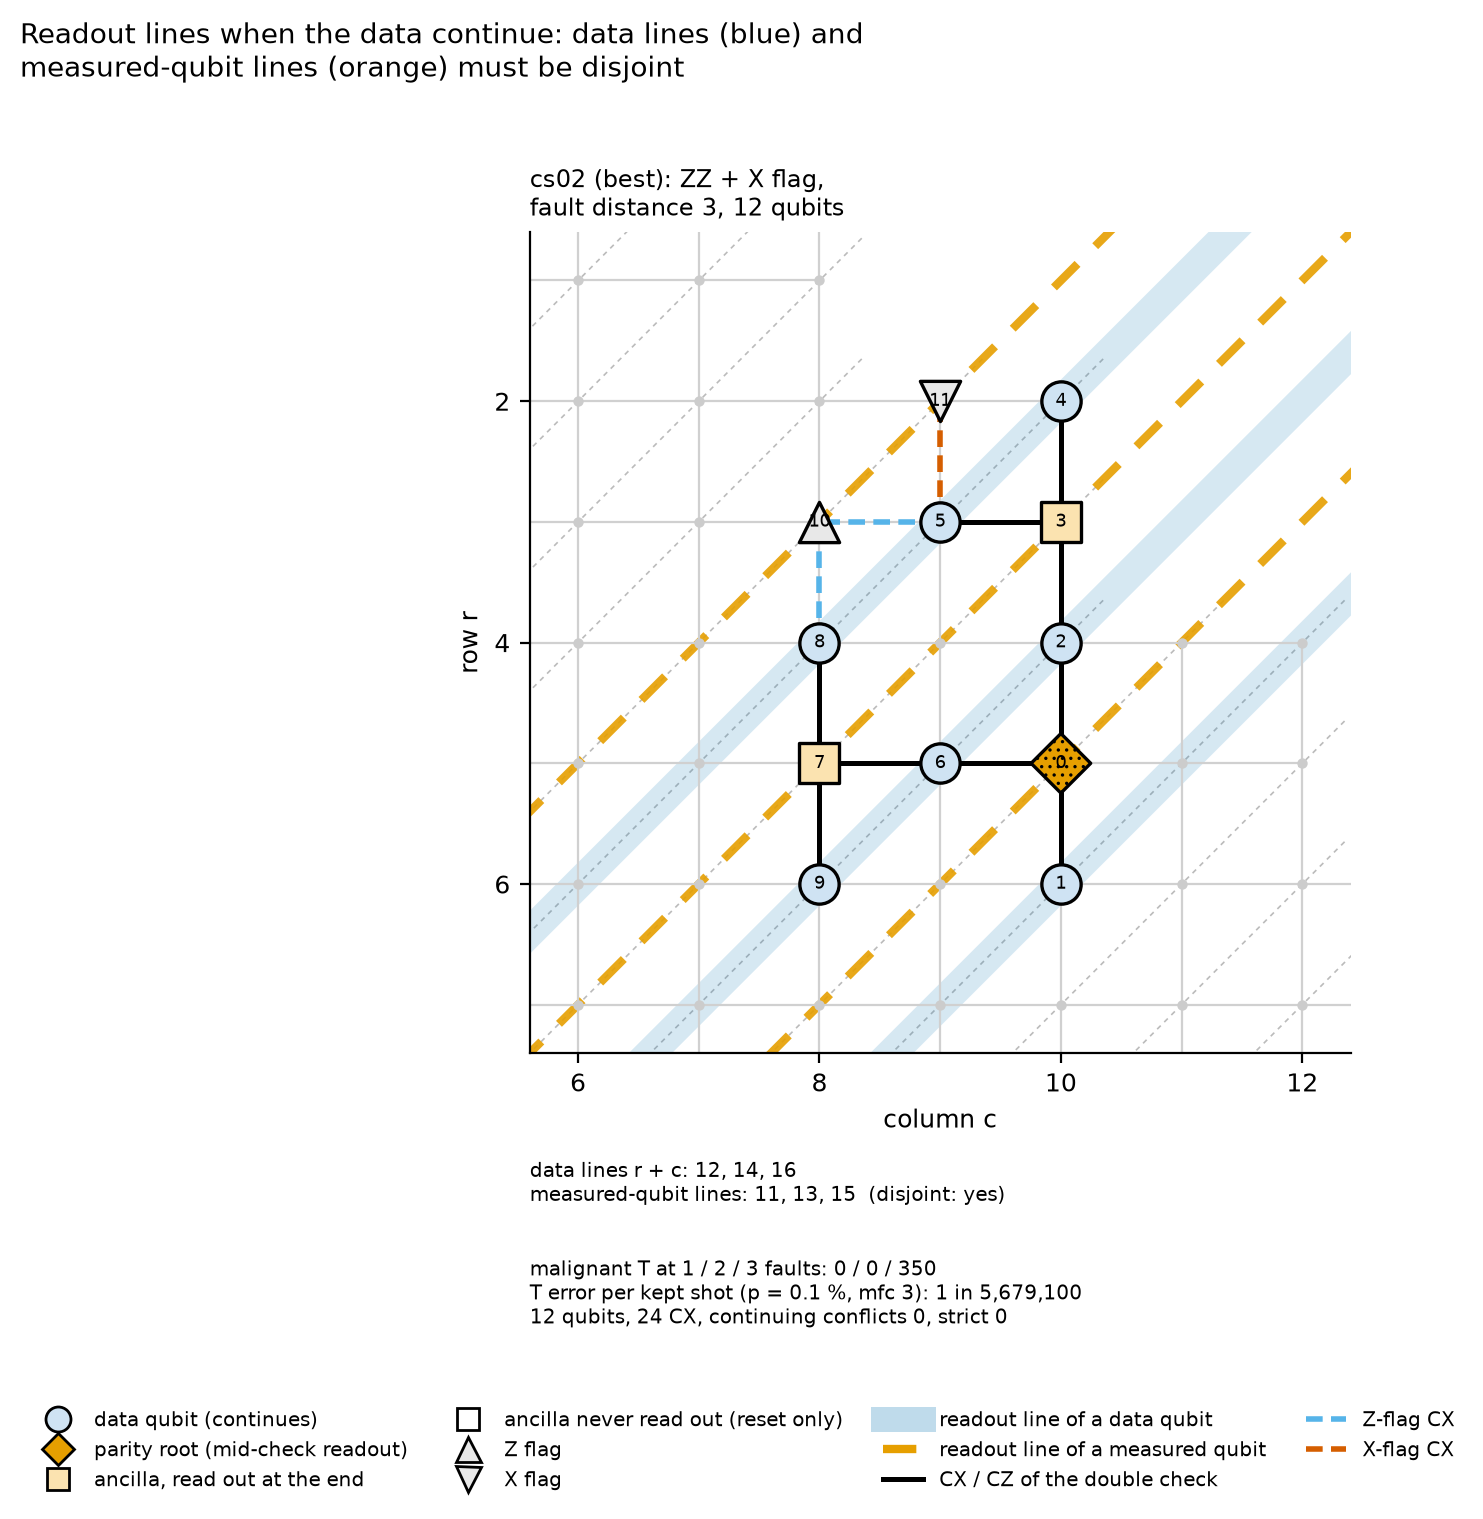
\includegraphics[width=\columnwidth]{figures/fig_layout_cs02.png}
\caption{\csz\ on Willow's square lattice. Circles: data qubits, which continue after the check; diamond: parity root, measured in the middle and at the end; squares: fold helpers read out at the end; triangles: the $Z$ (ZZ) flag and the $X$ flag. Black lines: CNOTs of the double check; dashed: flag CNOTs. Data qubits sit only on readout lines $r+c\in\{12,14,16\}$ (blue bands), every measured qubit on $\{11,13,15\}$ (orange), so the continuing-data rule holds with no conflict.}
\label{fig:layout}
\end{figure}

\begin{figure*}[t]
\centering
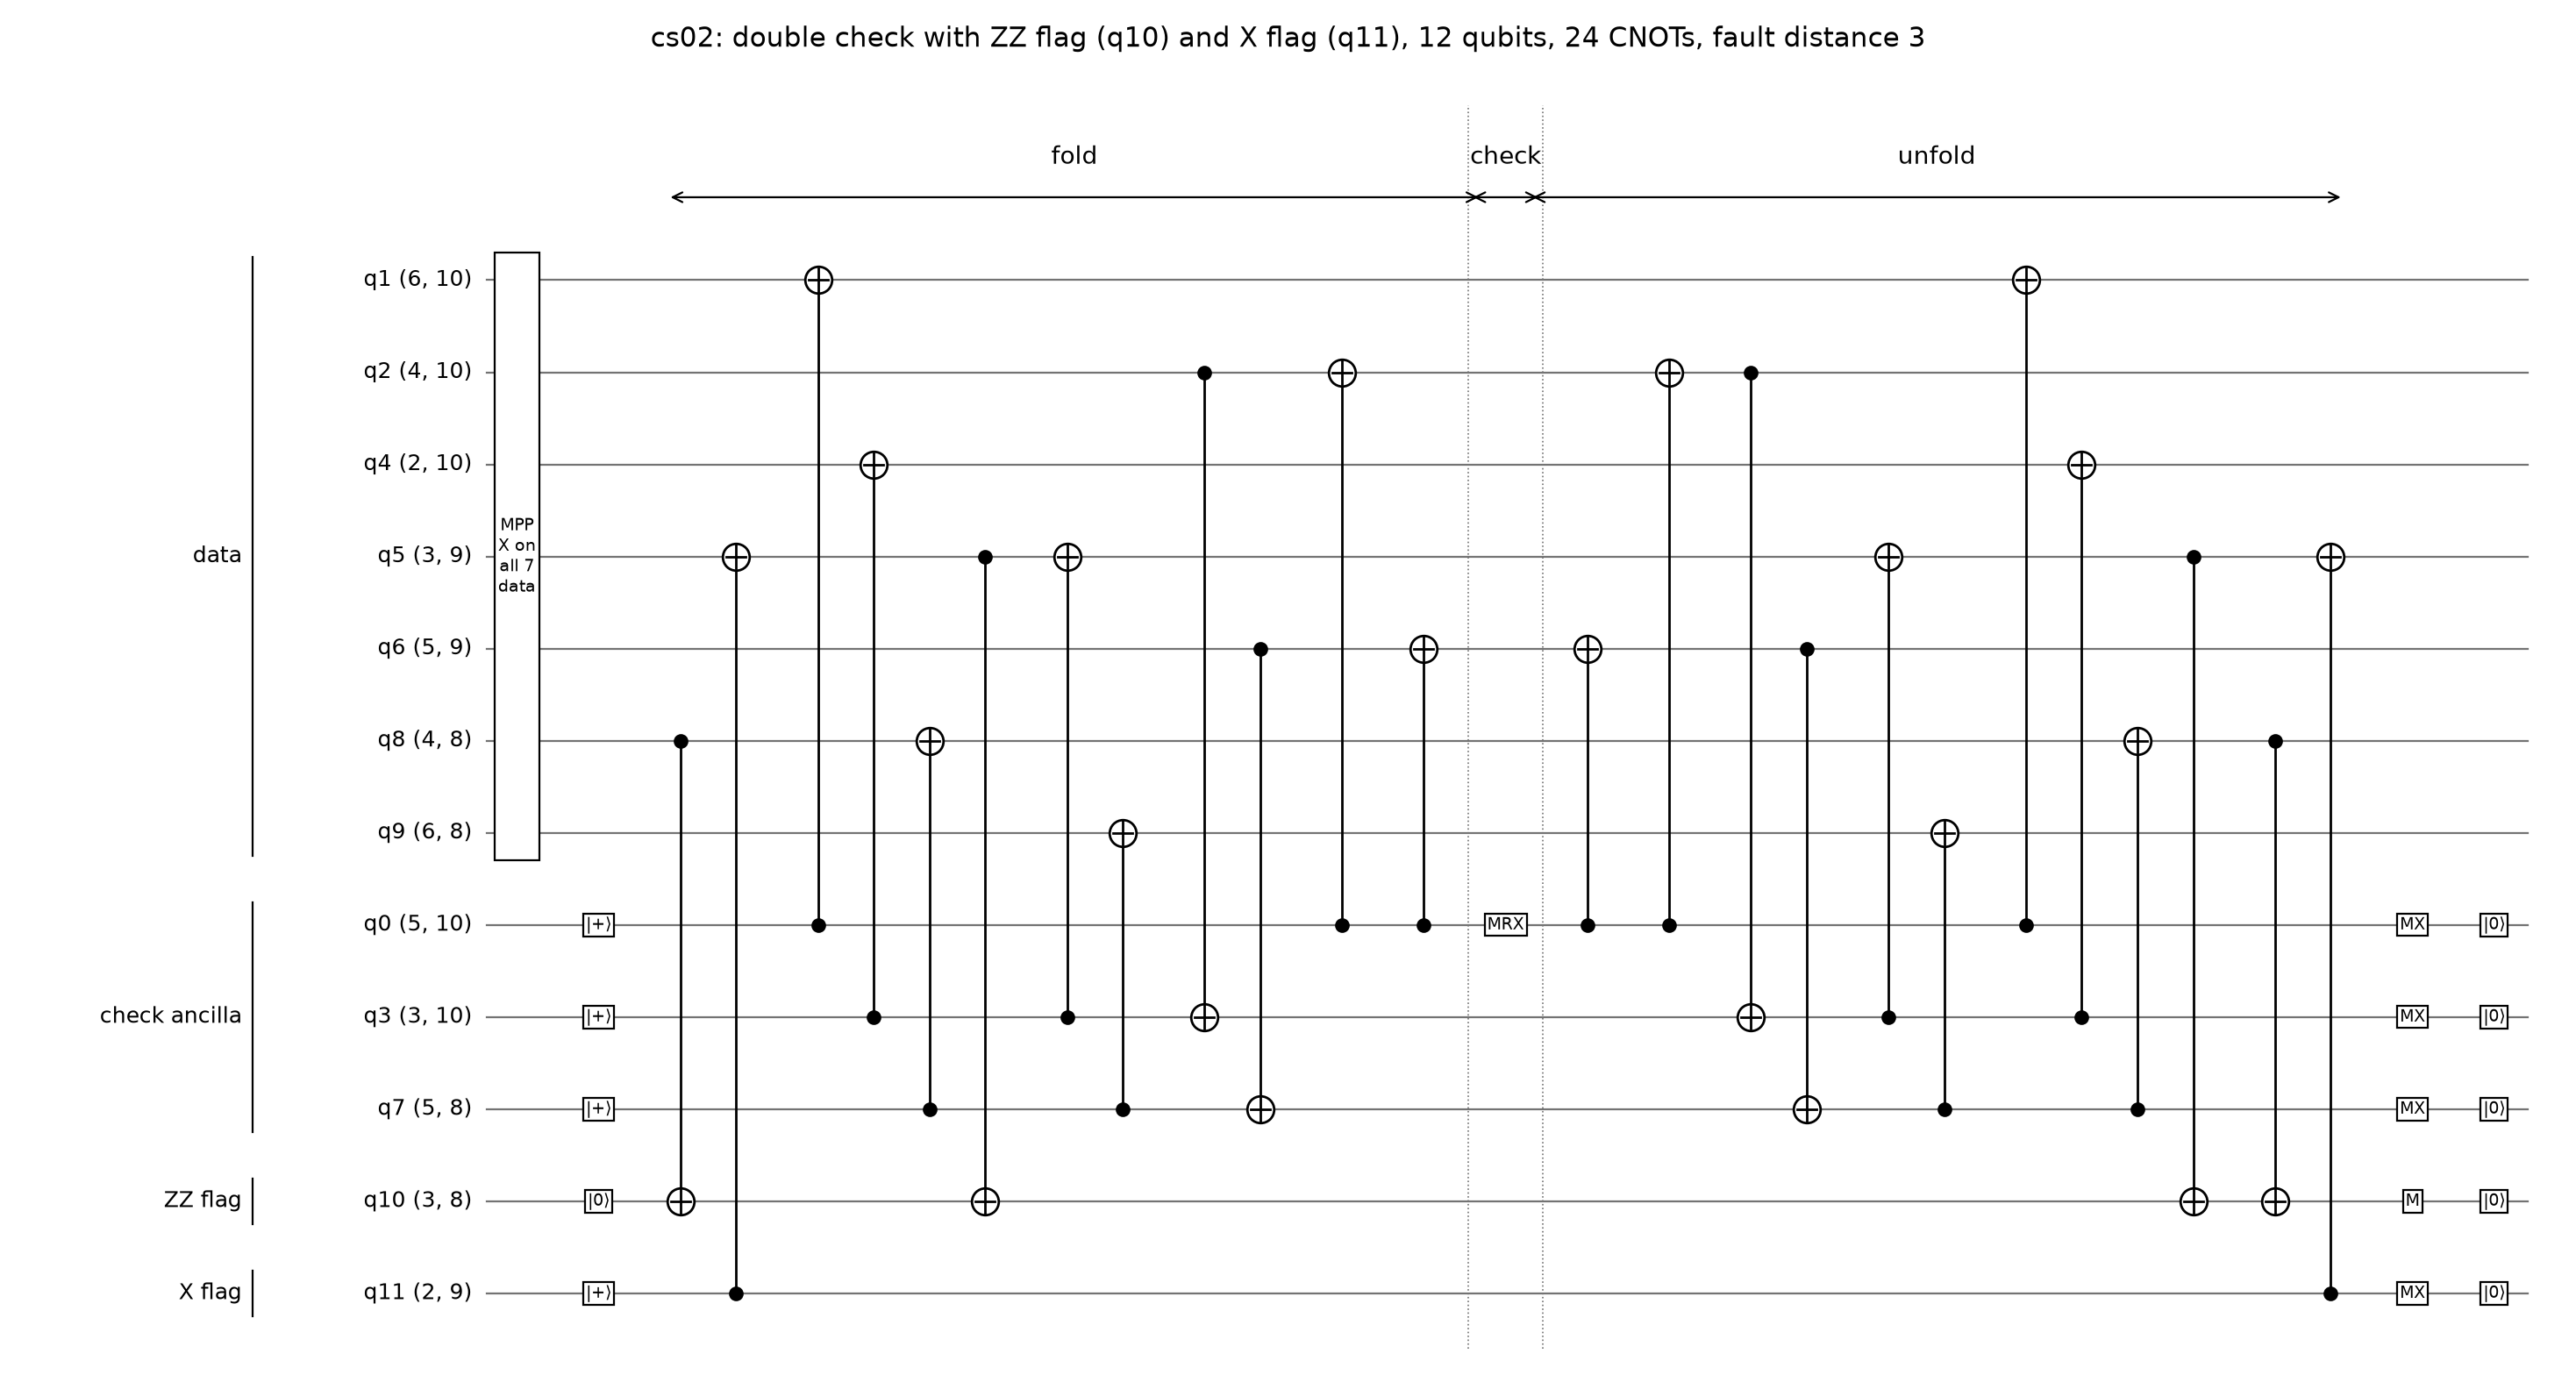
\includegraphics[width=0.92\textwidth]{figures/fig_circuit_cs02.png}
\caption{Gate-level circuit of \csz\ in CNOT form (the device circuit uses CZ and Hadamard gates). The fold collects $X_L$ onto the root $q_0$, which is measured ($\mathrm{MRX}$) between fold and unfold; helpers $q_3$, $q_7$, the root and the flags are read out at the end. The ZZ flag $q_{10}$ reads the parity $Z_8Z_5$ during the fold and the unfold and detects the $X$ hook errors that real $T$ gates turn into logical errors; the $X$ flag $q_{11}$ is coupled to $q_5$. The layers of physical $T^\dagger$ and $T$ gates before and after the circuit are not drawn.}
\label{fig:circuit}
\end{figure*}

Figures~\ref{fig:layout} and \ref{fig:circuit} show \csz.
It uses 12 qubits: 7 data qubits, the root, two fold helpers, a ZZ flag and an $X$ flag, and 24 CNOTs, as many qubits and two-qubit gates as \Gfour.
Every gate is between lattice neighbours and no qubit has more than three partners.
The data qubits occupy the even readout lines and all measured qubits the odd ones, so all measurements, including both flags, are allowed while the data continue.

Exhaustive enumeration with real $T$ gates gives $N_1=N_2=0$ and $N_3=350$ under uniform depolarising noise, so $\df=3$.
Fault injection in Google's QVM confirms that none of the 1,203 single faults and 13,041 fault pairs leaves a wrong $T$ state undetected (Table~\ref{tab:fd}).

\begin{table}[b]
\caption{Fault distance with real $T$ gates, from fault injection in Google's QVM (every single fault and every pair). The last column counts the configurations that are kept with a wrong $T$ state; QVM and \texttt{cliffordea} agree for every configuration.}
\label{tab:fd}
\begin{ruledtabular}
\begin{tabular}{lcccc}
circuit & 1 fault & 2 faults & wrong $T$ kept & $\df$\\
\colrule
\Gfour\ (Google, Fig.~2) & 1,018 & 11,781 & 7 & 2\\
\Gsix\ (Google, Fig.~4 rule) & 952 & 11,175 & 7 & 2\\
\csz\ (ours) & 1,203 & 13,041 & 0 & 3\\
\end{tabular}
\end{ruledtabular}
\end{table}

% =====================================================================================
\section{Results at distance 3}
\label{sec:results}
% =====================================================================================

\subsection{Google's simulator of Willow}

Table~\ref{tab:qvm} and Fig.~\ref{fig:qvm} give the main result: 8,000,000 shots per circuit in Google's QVM with real $T$ gates.
\csz\ keeps 75.2\,\% of the attempts (\Gfour: 75.1\,\%, \Gsix: 76.7\,\%) and lowers the error per kept $T$ state to 1 in 121,322, 5.8 times below \Gsix\ (95\,\% interval 4.2--8.1) and 6.6 times below \Gfour\ (4.7--9.1).
A stim simulation with our Pauli model of Willow's calibration gives the same factor (1 in 140,288 versus 1 in 24,121, 5.8 times).

\begin{table*}[t]
\caption{Main result: Google's QVM for Willow (\texttt{willow\_pink} noise model), real $T$ gates, 8,000,000 shots per circuit, identical ideal input and decode. Errors are counted among kept shots in the code space. Intervals are 95\,\%.}
\label{tab:qvm}
\begin{ruledtabular}
\begin{tabular}{lcccccc}
circuit & $\df$ & qubits & errors / kept & error per kept $T$ state & acceptance & gain over \Gsix\\
\colrule
\Gfour\ (Google, Fig.~2) & 2 & 12 & 239 / 4,411,869 & 1 in 18,460 (16,262--21,043) & 75.1\,\% & 0.89\\
\Gsix\ (Google, Fig.~4 rule) & 2 & 12 & 221 / 4,603,871 & 1 in 20,832 (18,259--23,876) & 76.7\,\% & 1\\
\csz\ (ours) & 3 & 12 & 42 / 5,095,514 & 1 in 121,322 (89,754--168,336) & 75.2\,\% & 5.8 (4.2--8.1)\\
\end{tabular}
\end{ruledtabular}
\end{table*}

\begin{figure*}[t]
\centering
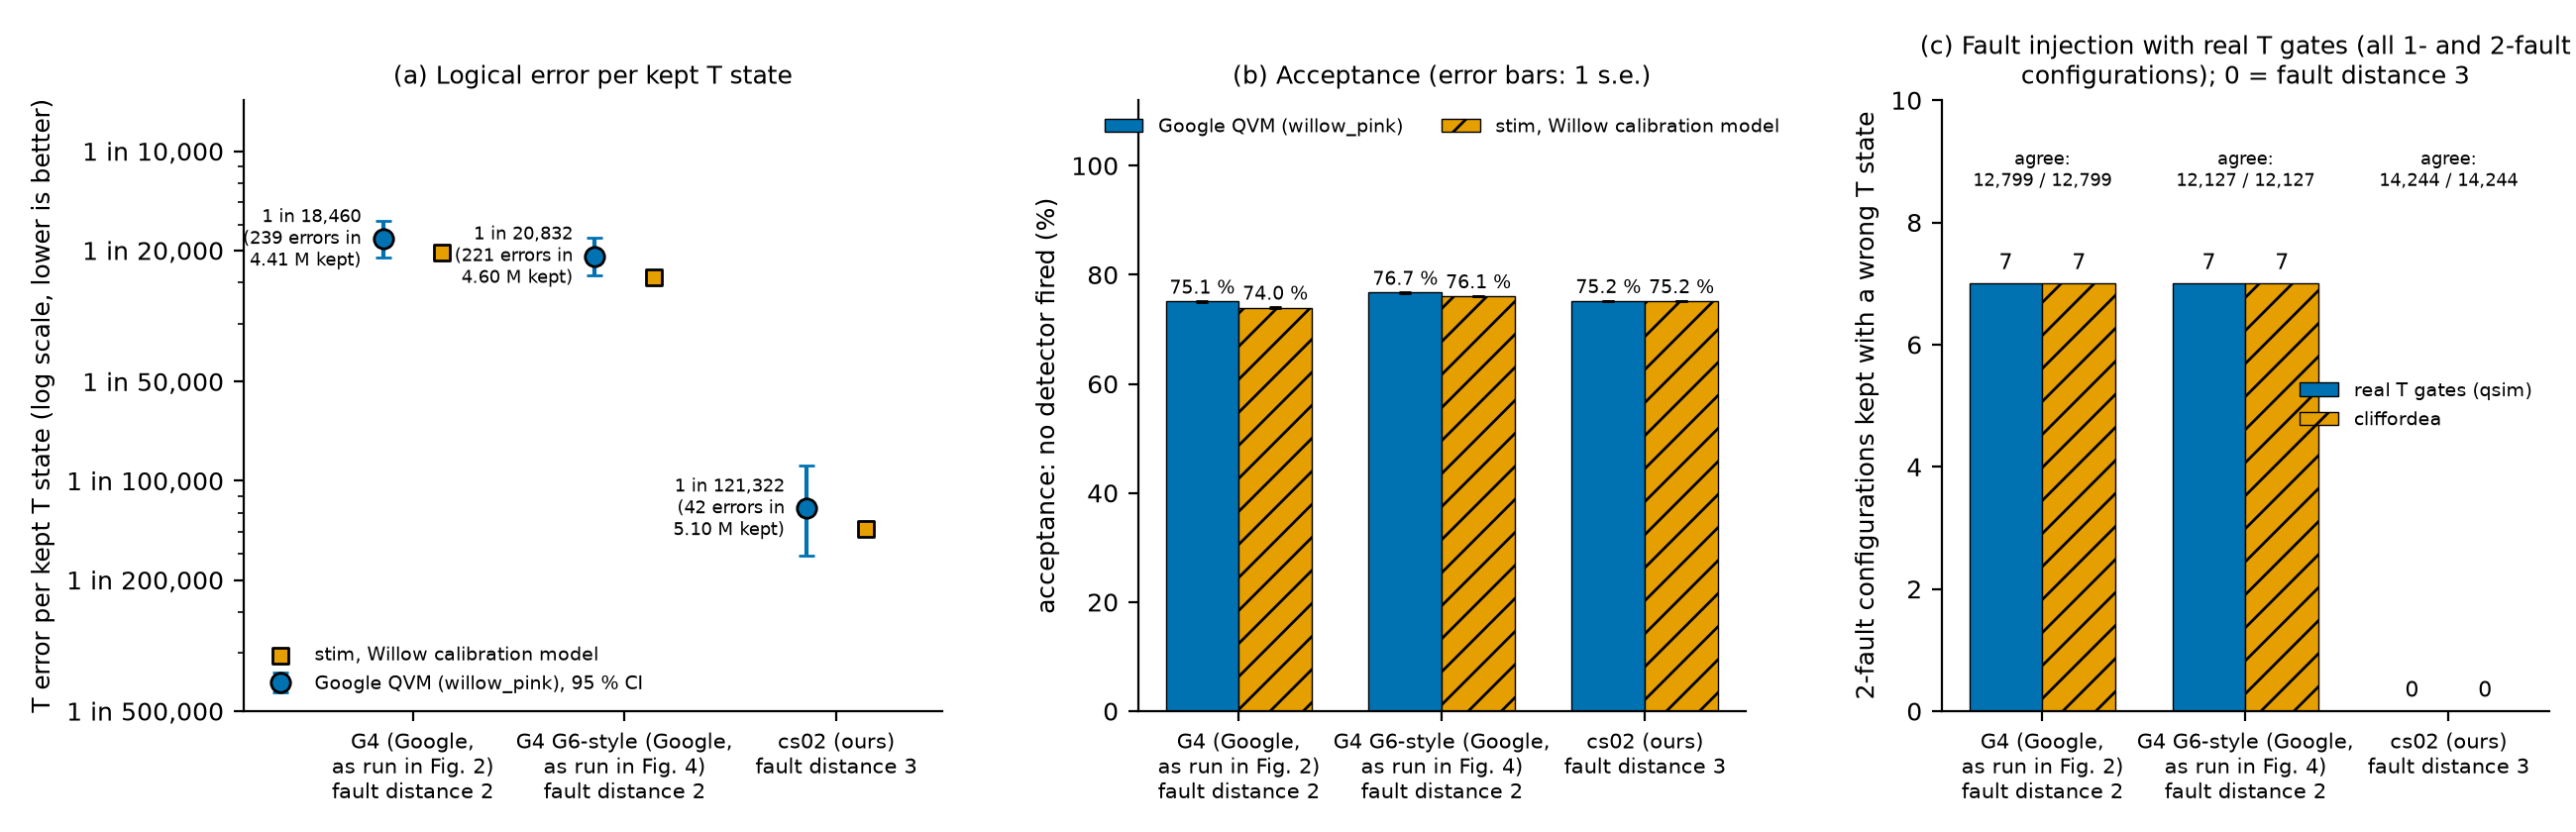
\includegraphics[width=\textwidth]{figures/fig_qvm_comparison.png}
\caption{Google's QVM, real $T$ gates. (a) Error per kept $T$ state with 95\,\% intervals (circles) and our stim Pauli model of Willow's calibration (squares). (b) Acceptance. (c) Fault injection: number of 2-fault configurations kept with a wrong $T$ state, QVM with real $T$ gates versus \texttt{cliffordea}; zero means fault distance three.}
\label{fig:qvm}
\end{figure*}

\subsection{Other noise models}

The improvement does not depend on the choice of simulator or noise model (Table~\ref{tab:models}).
Across uniform depolarising noise, SI1000 at Google's fitted strength, Willow's median specification and Willow's per-qubit calibration, \csz\ is 3.0--5.7 times better than \Gsix.
Its acceptance is 3--5 percentage points lower under the uniform, SI1000 and specification models, and within 1.5 points under the calibration model and the QVM.

\begin{table*}[t]
\caption{Error per kept $T$ state (acceptance) under five noise environments. QVM: sampling; other rows: exact enumeration with real $T$ up to 4 faults, acceptance from stim.}
\label{tab:models}
\begin{ruledtabular}
\begin{tabular}{lccc}
environment & \Gsix\ & \csz & gain\\
\colrule
Google QVM & 1 in 20,832 (76.7\,\%) & 1 in 121,322 (75.2\,\%) & 5.8\\
uniform, $p=0.1\,\%$ & 1 in 1,863,139 (93.4\,\%) & 1 in 5,504,576 (89.3\,\%) & 3.0\\
SI1000, $p=0.23\,\%$ & 1 in 209,037 (81.2\,\%) & 1 in 765,869 (78.3\,\%) & 3.7\\
Willow spec & 1 in 99,859 (81.2\,\%) & 1 in 336,453 (76.2\,\%) & 3.4\\
Willow calibration & 1 in 22,551 (74.8\,\%) & 1 in 128,163 (73.9\,\%) & 5.7\\
\end{tabular}
\end{ruledtabular}
\end{table*}

\subsection{Scaling with the noise strength}

Equation~\eqref{eq:eps} predicts $\varepsilon\propto p^{\df}$, and hence a gain
\begin{equation}
\frac{\varepsilon_{\Gsix}(p)}{\varepsilon_{\csz}(p)} \approx \frac{N_2^{\Gsix}\,p^2}{N_3^{\csz}\,p^3} \propto \frac{1}{p}
\label{eq:gain}
\end{equation}
that grows as the hardware improves.
Figure~\ref{fig:sweep} confirms this under SI1000 from $p=0.05\,\%$ to $0.5\,\%$.
The fitted log--log slopes for $p\le0.23\,\%$ are 3.04 for \csz\ and 2.17 for both Google circuits.
The gain rises from 2.2 times at $p=0.5\,\%$ and 3.7 times at Google's fitted $p=0.23\,\%$ to 13.7 times at $p=0.05\,\%$ (1 in 78,963,741 versus 1 in 5,772,643).

\begin{figure}[t]
\centering
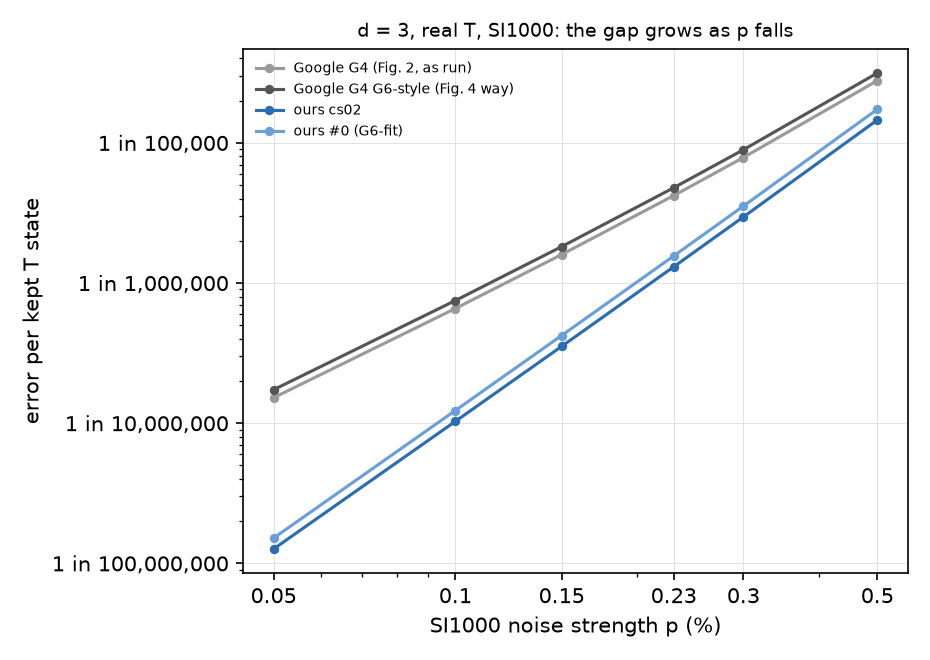
\includegraphics[width=\columnwidth]{figures/fig_si1000_sweep.png}
\caption{Error per kept $T$ state versus SI1000 strength $p$, real $T$ gates, exact enumeration. Google's circuits (grey) scale with slope 2.17, \csz\ (dark blue) with slope 3.04, as expected for fault distance 2 and 3. The light blue curve is \#0, our circuit that fits Google's grafting layout (Sec.~\ref{sec:g6fit}).}
\label{fig:sweep}
\end{figure}

\subsection{Chip placement}

The QVM comparison places each circuit at its own coordinates, and the two circuits occupy different regions of the chip.
To separate the circuit from the region, we evaluate every placement of each circuit on the 105-qubit lattice that satisfies the continuing-data rule (160 for \csz, 196 for \Gsix) under the per-qubit calibration model (Fig.~\ref{fig:positions}).
In the median, \csz\ reaches 1 in 111,425 and \Gsix\ 1 in 47,451, a gain of 2.3 times; the best placements are 1 in 314,443 and 1 in 175,366.
The spread over placements is large for both circuits: the worst placement of \csz\ (1 in 28,870) is worse than the best placement of \Gsix.
The choice of chip region therefore matters as much as the circuit, and both should be optimised together.

\begin{figure}[t]
\centering
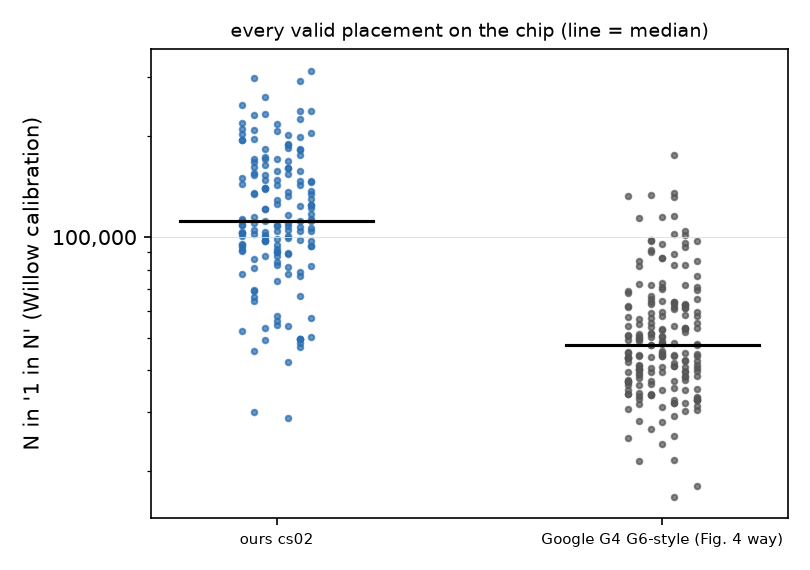
\includegraphics[width=\columnwidth]{figures/fig_chip_positions.png}
\caption{Error per kept $T$ state over all valid placements on Willow (per-qubit calibration model, continuing-data rule): \csz, 160 placements; \Gsix, 196 placements.}
\label{fig:positions}
\end{figure}

\subsection{Circuits that fit Google's grafting layout}
\label{sec:g6fit}

\csz\ does not use the qubits of Google's grafting experiment.
Restricting the search to that footprint gives nine fault-distance-3 circuits with 13--15 qubits.
In the QVM they are 2.4--4.1 times better than \Gsix; the best balance, circuit \#0 (13 qubits), reaches 1 in 70,284 at 71.4\,\% acceptance (3.4 times, interval 2.6--4.4).
These circuits can replace Google's double check in its grafting circuit without moving the surface-code patch.

% =====================================================================================
\section{Validation against Google's hardware data}
\label{sec:validation}
% =====================================================================================

Google released the circuits, raw measurements, detection events and processed observables of its experiments~\cite{RosenfeldData}.
We used them to check three links in our chain.

\paragraph{The baseline is the circuit that was run.}
\Gfour, built from the paper's circuit link, equals the released X-basis circuit of Fig.~2 at every time step, with the same detectors, observable and physical $T$ gates (7 $T$ and 7 $T^\dagger$, on the same seven data qubits). The circuits of Figs.~3 and~4 likewise match the corresponding links.

\paragraph{Our analysis reproduces the paper from the raw shots.}
From the raw measurements, our code recomputes Google's detection events and observables exactly, and Google's processed outputs for Figs.~2 and~3 equal our post-selected data in every setting.
The numbers printed in the paper follow (Table~\ref{tab:repro}).

\begin{table}[t]
\caption{Values recomputed by us from Google's released hardware shots, at the $T$ angle, compared with the paper~\cite{Rosenfeld2025}.}
\label{tab:repro}
\begin{ruledtabular}
\begin{tabular}{lcc}
quantity & ours, from the data & paper\\
\colrule
injection retention & 76.2\,\% & about 76\,\%\\
cultivation retention (Fig.~2) & 44.5\,\% & about 45\,\%\\
injection-only error (Fig.~3) & 1 in 224 & 1 in 227\\
full circuit error (Fig.~3) & 1 in 5,311 & 1 in 10,000--5,000\\
full circuit retention (Fig.~3) & 8.7\,\% & 8\,\%\\
\end{tabular}
\end{ruledtabular}
\end{table}

\paragraph{The simulator agrees with the hardware.}
We ran the released Fig.~2 circuit, with its real injection rotation and $T$ gates, in the QVM at ten injection angles.
The QVM follows the hardware retention over the whole angle sweep (Fig.~\ref{fig:validation}); at the $T$ angle it keeps 47.3\,\% of the attempts against 44.5\,\% on the hardware (a factor 1.06), and the cultivated state's logical expectation values agree.
The QVM is therefore slightly optimistic in absolute terms, as expected for a model without leakage, but it describes the circuit Google ran.

We also compared our SI1000 implementation with Google's released simulated shots of the same circuit.
At the stated $p=0.30\,\%$ every detector fires $0.83\pm0.03$ times as often in our simulation as in Google's, so our implementation is uniformly about 1.2 times weaker; at $p=0.36\,\%$ the detector rates match within 2\,\% and the retention near the $T$ angle within 2\,\%.
Since all circuits in Sec.~\ref{sec:results} are compared within one implementation, this convention difference shifts absolute values, not the comparison.

\begin{figure}[t]
\centering
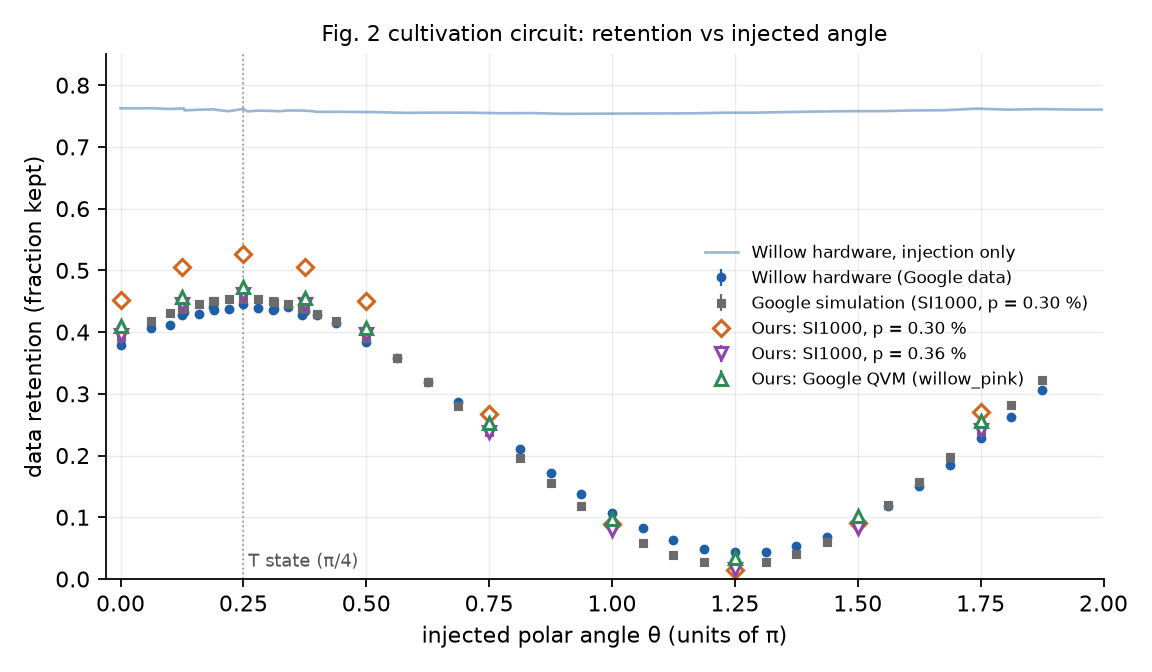
\includegraphics[width=\columnwidth]{figures/fig_validation_retention.png}
\caption{Retention of Google's Fig.~2 cultivation circuit versus injected angle: Willow hardware (Google's released data), Google's released simulation, our SI1000 at $p=0.30\,\%$ and $0.36\,\%$, and our run of Google's QVM. The line is the hardware retention after injection only.}
\label{fig:validation}
\end{figure}

% =====================================================================================
\section{Extension to distance 5}
\label{sec:d5}
% =====================================================================================

At distance 5 the published design is the double check of Gidney \emph{et al.}~\cite{Gidney2024cultivation} (38 qubits, 74 two-qubit gates).
With real $T$ gates its fault distance is 3 (3 malignant triples and 601 malignant 4-fault configurations), and none of its 62 rigid placements on Willow satisfies the readout rule.
Google did not run a distance-5 double check.
The only available baseline therefore does not run on the device; we report it as the reference design.

We applied the same method to the 19-qubit code: the root alone on its readout line, an as-soon-as-possible fold of 19 leaves, a search over code labellings, and greedy nearest-neighbour flags.
The search returned 41 circuits with 23--33 qubits that fit Willow and have fault distance four with real $T$ gates; most need no flag.
Table~\ref{tab:d5} compares the best of them with the reference design (exact enumeration up to four faults, acceptance from stim).
The gain is 3.0--5.4 times and our circuits keep more attempts (57\,\% against 47\,\% at SI1000, $p=0.23\,\%$).
Sampling with Clifft~\cite{Clifft}, a second simulator with real $T$ gates, agrees with the enumeration within the statistical intervals for the reference design and our two best circuits.

\begin{table*}[t]
\caption{Distance 5, real $T$ gates: error per kept $T$ state (acceptance). Reference: Gidney \emph{et al.}'s design~\cite{Gidney2024cultivation} (fault distance 3; not placeable on Willow under the readout rule). Ours: \#1035 (33 qubits, fault distance 4). Exact enumeration up to four faults.}
\label{tab:d5}
\begin{ruledtabular}
\begin{tabular}{lccc}
environment & reference & ours & gain\\
\colrule
SI1000, $p=0.23\,\%$ & 1 in 140.6\,M (46.7\,\%) & 1 in 422.7\,M (57.1\,\%) & 3.0\\
SI1000, $p=0.1\,\%$ & 1 in 2.19\,G (71.7\,\%) & 1 in 11.8\,G (78.2\,\%) & 5.4\\
Willow spec & 1 in 32.3\,M (44.0\,\%) & 1 in 148.4\,M (55.8\,\%) & 4.6\\
Willow calibration & 1 in 8.55\,M (39.2\,\%) & 1 in 32.3\,M (52.9\,\%) & 3.8\\
\end{tabular}
\end{ruledtabular}
\end{table*}

% =====================================================================================
\section{Discussion and limitations}
\label{sec:limitations}
% =====================================================================================

\paragraph{What is shown.}
A double check with the full fault distance three under real $T$ gates exists within Willow's coupling graph, uses no more qubits or two-qubit gates than the circuit run on hardware, and remains valid when the cultivated state continues.
In every simulator and noise model we tried it lowers the error per kept $T$ state, by a factor that grows as $1/p$.

\paragraph{Simulation only.}
All results on \csz\ are simulations. We tied the simulator to the hardware through Google's released data (Sec.~\ref{sec:validation}), but leakage, coherent errors and crosstalk are not modelled, and the QVM uses a 2024 median calibration rather than the calibration of a given day.

\paragraph{The readout-line model.}
The rule $\ell=r+c$ with dephasing of the whole line is our model of Willow's readout constraint. It agrees with the published layout but should be confirmed against the device's actual readout multiplexing.

\paragraph{Chip region.}
Part of the 5.8-times gain at the as-published placements comes from the chip region; over all valid placements the median gain is 2.3 times, and the region matters as much as the circuit.

\paragraph{Scope.}
We analyse the double check alone, from an ideal encoded input to an ideal decode. Injection, escape and grafting are unchanged and common to both circuits; an end-to-end simulation including them is future work.

\paragraph{Distance 5.}
The distance-5 circuits reach fault distance four, not five, the reference design cannot run on the device, the continuing-data rule has not yet been imposed at distance 5, and the enumeration is truncated at four faults.

\paragraph{Related work.}
Garner \emph{et al.}~\cite{Garner2026} adapt Google's double check to a square-lattice IBM device for lattice surgery; they do not address the fault distance. Comb~\cite{Simsek2026} verifies fault tolerance of CNOT+$T$ preparation circuits and could serve as a further independent check.

% =====================================================================================
\section{Conclusion}
% =====================================================================================

The double check at the core of magic state cultivation loses one unit of fault distance with physical $T$ gates, including in the circuit demonstrated on Willow.
Treating the device's coupling and readout constraints as part of the design problem, we found \csz, a nearest-neighbour double check of the same size as Google's that restores fault distance three, keeps nearly the same acceptance, and lowers the error per kept $T$ state 5.8 times in Google's simulator of Willow, with a gain that grows as the hardware improves.
The circuit can be run on the existing device with no hardware change.
The next steps are a hardware run, an end-to-end simulation with injection and grafting, and fault distance five at distance 5.

\begin{acknowledgments}
\todo{Acknowledgments and funding.} We thank Google Quantum AI for releasing the circuits and data of Ref.~\cite{Rosenfeld2025}.
\end{acknowledgments}

\section*{Data and code availability}
\todo{Repository link.} Google's data: Ref.~\cite{RosenfeldData}.

\bibliography{references}

\end{document}
